\documentclass[12pt,a4paper]{article}
% \usepackage[portuges]{babel}
% \usepackage[utf8]{inputenc}
% \usepackage[T1]{fontenc}
\usepackage{hyperref}
\usepackage{url}
\usepackage{graphicx}
\usepackage{float}
\usepackage{enumerate}
\usepackage{makeidx}
\usepackage{booktabs}
\usepackage{longtable}
\usepackage{pdfpages}
\usepackage{a4wide}
\usepackage{xcolor}
\usepackage{indentfirst}

\setlength\oddsidemargin{0.3in}
\setlength\evensidemargin{-0.3in}
\setlength\headsep{15pt}
\setlength\footskip{30pt}

\usepackage{fontspec}
\defaultfontfeatures{Mapping=tex-text}
\setmainfont[
  Extension=.ttf,
  Path=font/,
  Scale=1.00,
  BoldFont={NewsGotTMed Regular},
  ItalicFont={NewsGoth Lt BT Light},
  ItalicFeatures={FakeSlant},
  AutoFakeSlant=0.3,
  BoldItalicFeatures=FakeSlant, 
]{NewsGotT Regular Fixed}

%Line Spacing
\usepackage{xspace}
\usepackage{setspace}
\onehalfspacing

% Language definitions
\usepackage{polyglossia}
\setmainlanguage{portuges}



% environment created for organization purposes, only.
\newenvironment{TODO}{%
  \color{blue} \itshape \begin{itemize}
}{%
  \end{itemize}
}

%---------------------------------------

% our addimage command
\newcommand{\addimg}[1]{%
  \begin{center}
    \includegraphics[width=0.75\textwidth]{#1}
  \end{center}
}

\newcommand{\RowStretch}[1]{\renewcommand{\arraystretch}{#1}}


%----------------------------------------------------------

\begin{document}

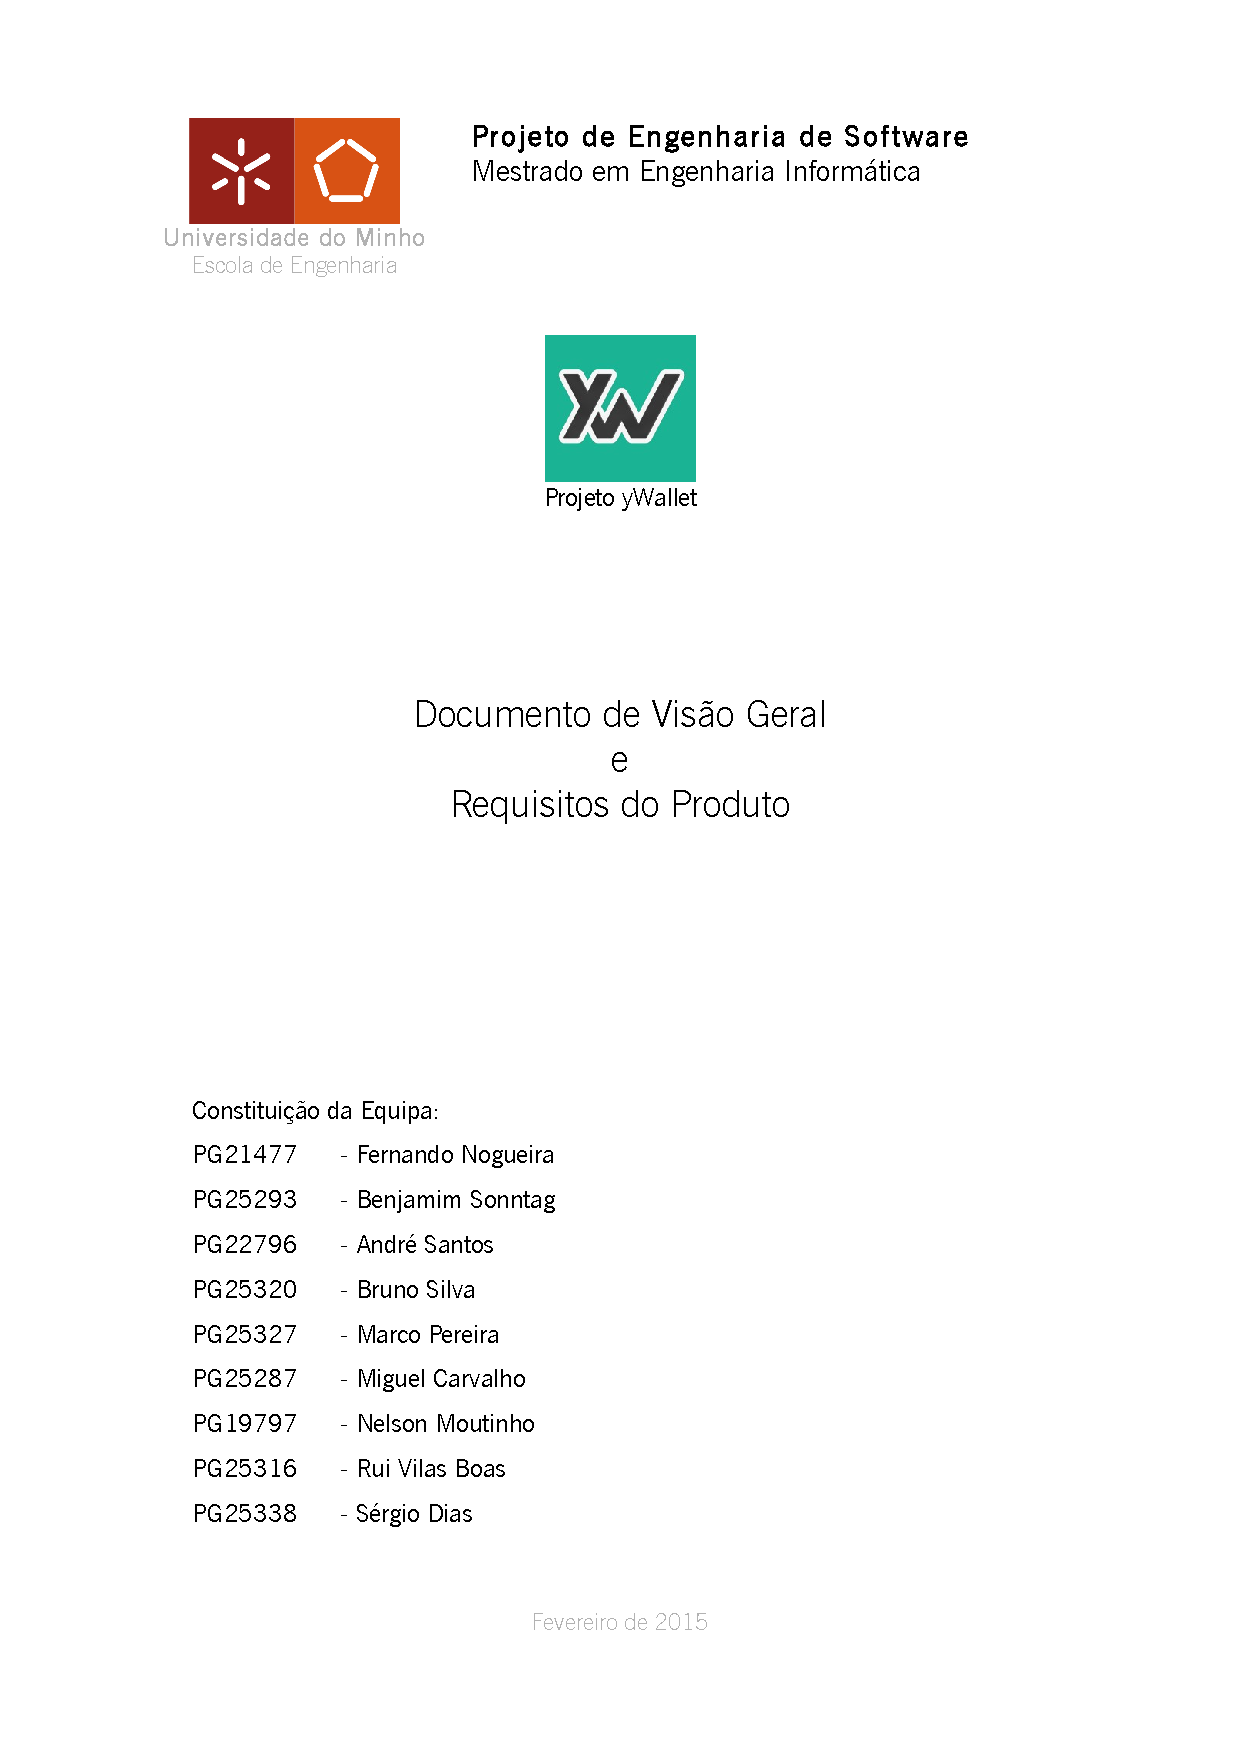
\includepdf[pages=-]{capa}

\section*{Introdução}

  Neste documento descreve-se como se procede à instalação do sistema yWallet. São descritos os pré-requisitos e os passos necessários para efetuar a instalação, assim como as configurações mínimas para a execução da aplicação e possíveis testes a efetuar no fim da instalação.

\section*{Pré-requisitos}

  Nesta secção é descrita uma lista de pré-requisitos que é necessário cumprir antes da instalação começar.

\begin{table}[h!]
\begin{tabular}{|l|l|}
\hline
Sistema Operativo & Ubuntu Server 14.04.1 LTS                                                  \\ \hline
Software          & Ruby 2.2.0; Bundler, Rails 4.2.0; Git 2.2.2                                \\ \hline
Base de Dados     & PostgreSQL 9.4                                                             \\ \hline
Hardware          & 700 MHz processor; 512 MB RAM; 100 GB of hard-drive space; Internet Access \\ \hline
\end{tabular}
\end{table}

\section*{Instalação}

  Assim que os pré-requisitos estiverem cumpridos, o processo de instalação pode começar. Nesta secção descrevem-se os passos necessários para instalar a aplicação yWallet.

  Primeiro é necessário criar um utilizador de sistema:

  \begin{verbatim}
      useradd -d /home/ywallet -m ywallet
      echo “ywallet ALL=(ALL:ALL) ALL” >> /etc/sudoers
      passwd ywallet
  \end{verbatim}

  Uma vez definida a password, faz-se login com o novo utilizador:

  \begin{verbatim}
      su - ywallet
  \end{verbatim}

  Tendo a sessão iniciada, passa-se ao download do código e instalação da aplicação:

  \begin{verbatim}
      git clone https://github.com/ywallet/ywallet-backend \\
      /home/ywallet/ywallet-app
      cd ywallet
      bundle install
  \end{verbatim}

  Por fim prepara-se a base de dados com o comando:

  \begin{verbatim}
      rake db:reset
  \end{verbatim}

  No fim destes passos a aplicação encontra-se pronta para executar.


\section*{Execução}

  No final da instalação é esperado existir uma pasta em “/home/ywallet/ywallet” com o código da aplicação.

  Para executar a aplicação é apenas necessário fazer o seguinte:


  \begin{verbatim}
      cd /home/ywallet/ywallet-app
      rails server -e production -d
  \end{verbatim}

  Com isto a aplicação começará a executar em background. O log da aplicação com possíveis mensagens de erro e/ou aviso pode ser visto em \verb!"/home/ywallet/ywallet-app/log/production.log"!.



\section*{Desinstalação}

  Nesta secção descrevem-se os passos necessários para desinstalar a aplicação, caso seja necessário.

  Antes de desinstalar é necessário parar a aplicação:


  \begin{verbatim}
      kill -INT $(cat /home/ywallet/ywallet-app/tmp/pids/server.pid)
  \end{verbatim}

  Com a aplicação parada é então possível desinstalar fazendo:


  \begin{verbatim}
      userdel ywallet
      rm -rf /home/ywallet
  \end{verbatim}

\end{document}
